
\documentclass[a4paper,11pt]{article}
\usepackage{geometry}
\geometry{margin=2cm}
\usepackage{booktabs}
\usepackage{graphicx}
\usepackage{amsmath}
\usepackage{siunitx}
\usepackage{caption}
\usepackage{times}
\usepackage[utf8]{inputenc}
\usepackage{tocloft}
\usepackage{rotating} % Untuk mendukung landscape

\title{Spectral Simulation Report}
\author{Automated Analysis}
\date{\today}

\begin{document}

\maketitle
\tableofcontents
\clearpage

\section{Introduction}
This report presents the results of spectral simulations derived from HDF5 dataset analysis. Each sample includes a spectral plot (combined into a single PDF page) and a detailed table summarizing the initial composition, actual positions, total pixels, and signal-to-noise ratio (SNR), along with simulation parameters such as temperature and electron density.


\section{Sample: 18440}
\subsection{Simulation Parameters}
\begin{table}[h!]
    \centering
    \begin{tabular}{ll}
        \toprule
        \textbf{Parameter} & \textbf{Value} \\
        \midrule
        Temperature ($T$) & 5505 \,\si{K} \\
        Electron Density ($n_e$) & 5.72e+17 \,\si{cm^-3} \\
        Total Pixels & 4096 \\
        Signal-to-Noise Ratio (SNR) & 33.22 \\
        \bottomrule
    \end{tabular}
    \caption{Simulation parameters and additional metrics for sample 18440.}
    \label{tab:params_18440}
\end{table}

\subsection{Composition Analysis}
\begin{table}[h!]
    \centering
    \begin{tabular}{lcc}
        \toprule
        \textbf{Element} & \textbf{Initial Composition (\%)} & \textbf{Actual Positions} \\
        \midrule
        Al & 9.99 & 125.0 \\
        Ar & 8.33 & 246.0 \\
        C & 0.00 & 0.0 \\
        Ca & 7.73 & 150.0 \\
        Cl & 7.76 & 12.0 \\
        Co & 0.00 & 0.0 \\
        Cr & 1.54 & 397.0 \\
        Fe & 8.43 & 2054.0 \\
        Mg & 4.59 & 139.0 \\
        Mn & 10.22 & 466.0 \\
        N & 0.00 & 0.0 \\
        Na & 7.62 & 330.0 \\
        Ni & 8.42 & 478.0 \\
        O & 7.91 & 8.0 \\
        S & 0.52 & 25.0 \\
        Si & 6.94 & 106.0 \\
        Ti & 10.01 & 1181.0 \\
        background & N/A & 1284.0 \\

        \midrule
        \textbf{Total Positions} & & 7001.0 \\
        \bottomrule
    \end{tabular}
    \caption{Composition analysis for sample 18440.}
    \label{tab:comp_18440}
\end{table}

\subsection{Spectral Plot}
\begin{figure}[h!]
    \centering
    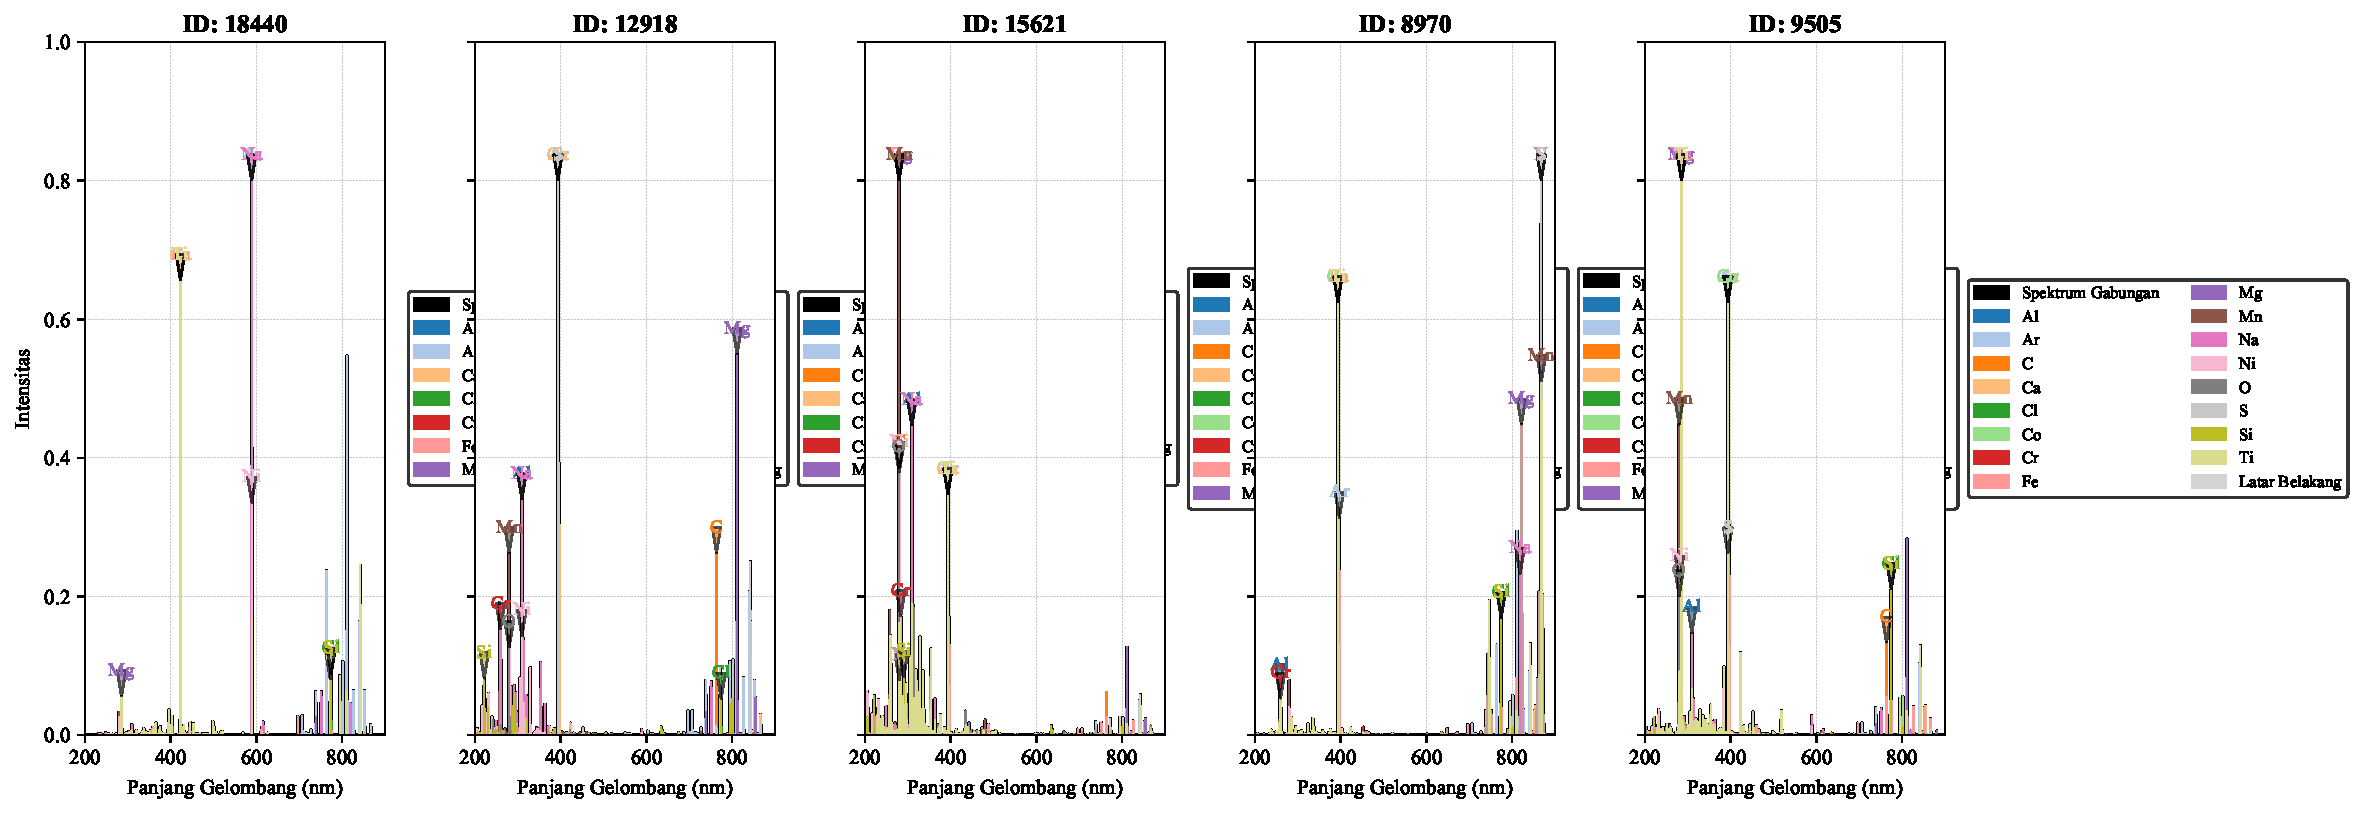
\includegraphics[width=\textwidth]{spectral_plots.pdf}
    \caption{Spectral simulation plots for all samples in a single landscape page.}
    \label{fig:spectrum_all}
\end{figure}

\clearpage

\section{Sample: 12918}
\subsection{Simulation Parameters}
\begin{table}[h!]
    \centering
    \begin{tabular}{ll}
        \toprule
        \textbf{Parameter} & \textbf{Value} \\
        \midrule
        Temperature ($T$) & 10657 \,\si{K} \\
        Electron Density ($n_e$) & 1.07e+17 \,\si{cm^-3} \\
        Total Pixels & 4096 \\
        Signal-to-Noise Ratio (SNR) & 33.37 \\
        \bottomrule
    \end{tabular}
    \caption{Simulation parameters and additional metrics for sample 12918.}
    \label{tab:params_12918}
\end{table}

\subsection{Composition Analysis}
\begin{table}[h!]
    \centering
    \begin{tabular}{lcc}
        \toprule
        \textbf{Element} & \textbf{Initial Composition (\%)} & \textbf{Actual Positions} \\
        \midrule
        Al & 10.82 & 462.0 \\
        Ar & 11.82 & 727.0 \\
        C & 1.64 & 259.0 \\
        Ca & 7.44 & 150.0 \\
        Cl & 4.39 & 28.0 \\
        Co & 0.00 & 0.0 \\
        Cr & 2.56 & 397.0 \\
        Fe & 0.00 & 0.0 \\
        Mg & 2.95 & 354.0 \\
        Mn & 10.93 & 706.0 \\
        N & 0.00 & 0.0 \\
        Na & 8.99 & 330.0 \\
        Ni & 13.88 & 478.0 \\
        O & 9.87 & 196.0 \\
        S & 8.27 & 228.0 \\
        Si & 6.45 & 223.0 \\
        Ti & 0.00 & 0.0 \\
        background & N/A & 1383.0 \\

        \midrule
        \textbf{Total Positions} & & 5921.0 \\
        \bottomrule
    \end{tabular}
    \caption{Composition analysis for sample 12918.}
    \label{tab:comp_12918}
\end{table}

\subsection{Spectral Plot}
\begin{figure}[h!]
    \centering
    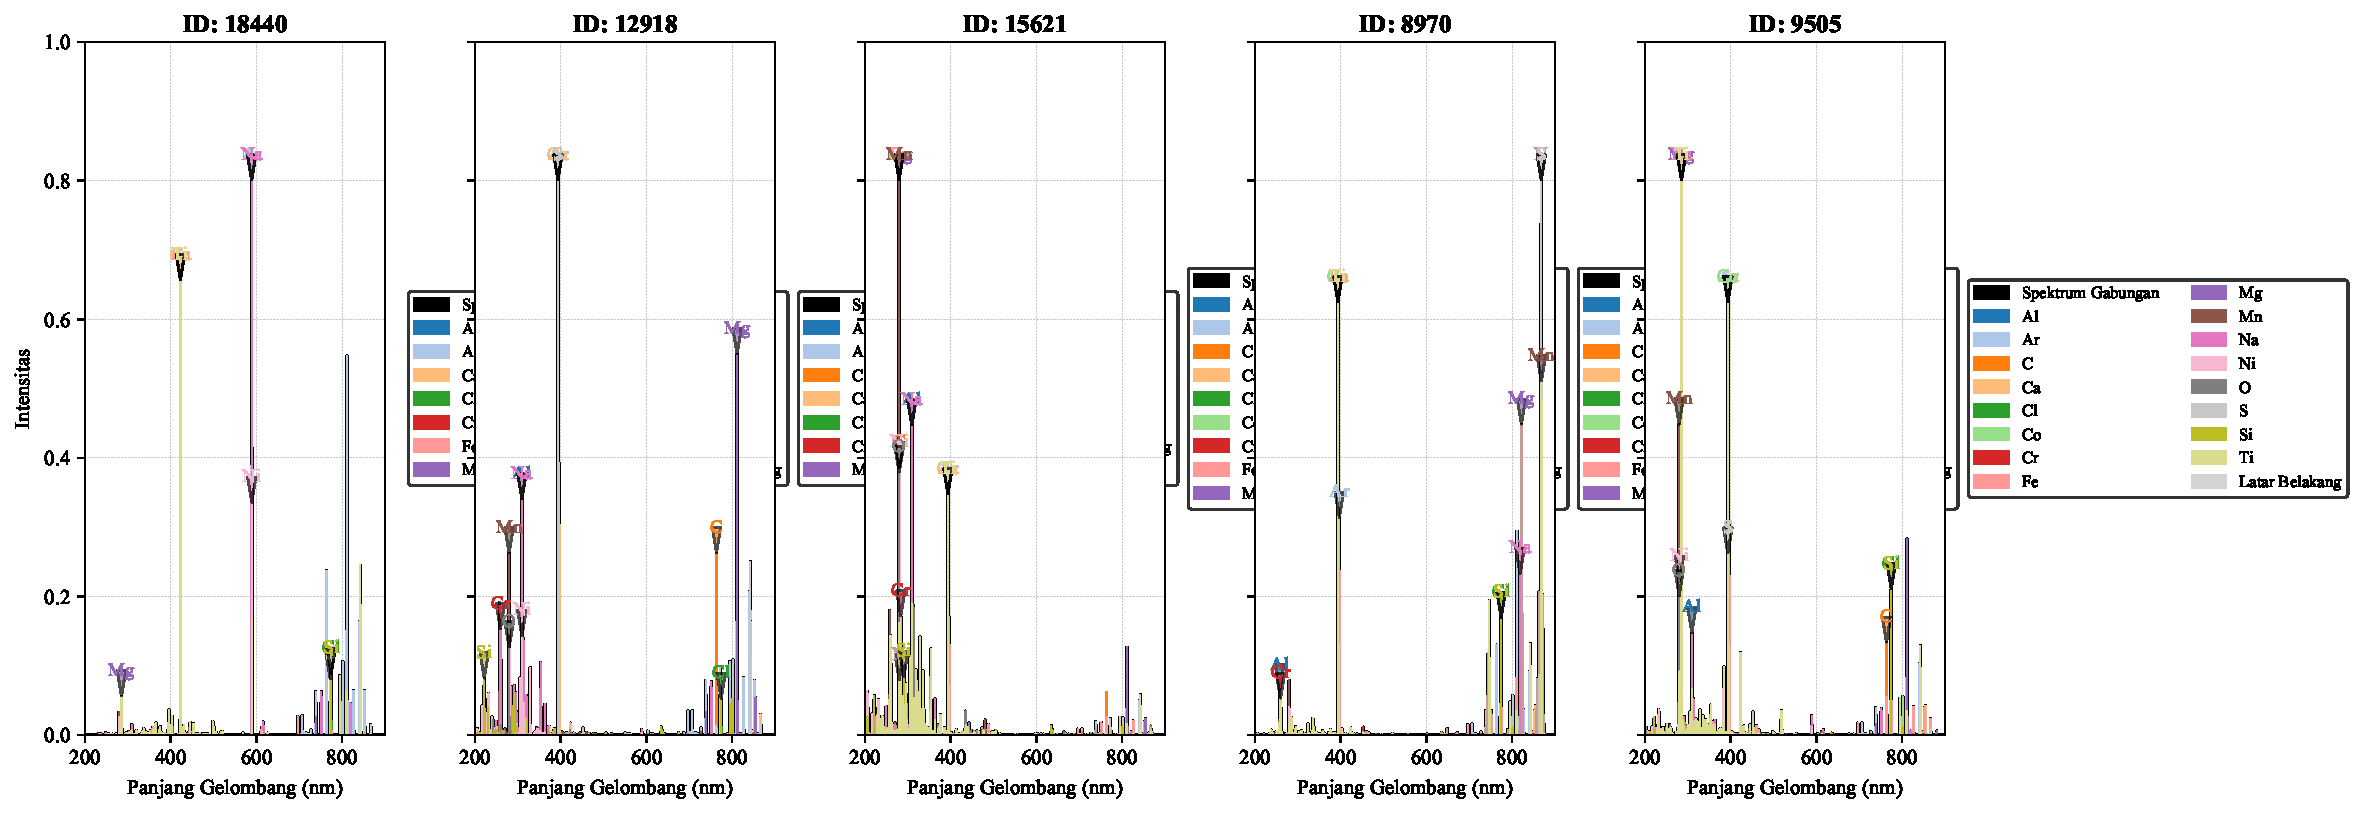
\includegraphics[width=\textwidth]{spectral_plots.pdf}
    \caption{Spectral simulation plots for all samples in a single landscape page.}
    \label{fig:spectrum_all}
\end{figure}

\clearpage

\section{Sample: 15621}
\subsection{Simulation Parameters}
\begin{table}[h!]
    \centering
    \begin{tabular}{ll}
        \toprule
        \textbf{Parameter} & \textbf{Value} \\
        \midrule
        Temperature ($T$) & 13485 \,\si{K} \\
        Electron Density ($n_e$) & 1.83e+16 \,\si{cm^-3} \\
        Total Pixels & 4096 \\
        Signal-to-Noise Ratio (SNR) & 35.94 \\
        \bottomrule
    \end{tabular}
    \caption{Simulation parameters and additional metrics for sample 15621.}
    \label{tab:params_15621}
\end{table}

\subsection{Composition Analysis}
\begin{table}[h!]
    \centering
    \begin{tabular}{lcc}
        \toprule
        \textbf{Element} & \textbf{Initial Composition (\%)} & \textbf{Actual Positions} \\
        \midrule
        Al & 2.45 & 462.0 \\
        Ar & 8.50 & 727.0 \\
        C & 4.37 & 749.0 \\
        Ca & 4.22 & 150.0 \\
        Cl & 5.23 & 35.0 \\
        Co & 4.54 & 1404.0 \\
        Cr & 10.84 & 397.0 \\
        Fe & 3.14 & 2737.0 \\
        Mg & 7.21 & 354.0 \\
        Mn & 10.51 & 706.0 \\
        N & 1.62 & 636.0 \\
        Na & 11.18 & 322.0 \\
        Ni & 5.91 & 478.0 \\
        O & 4.45 & 348.0 \\
        S & 2.83 & 228.0 \\
        Si & 5.15 & 223.0 \\
        Ti & 7.83 & 1189.0 \\
        background & N/A & 350.0 \\

        \midrule
        \textbf{Total Positions} & & 11495.0 \\
        \bottomrule
    \end{tabular}
    \caption{Composition analysis for sample 15621.}
    \label{tab:comp_15621}
\end{table}

\subsection{Spectral Plot}
\begin{figure}[h!]
    \centering
    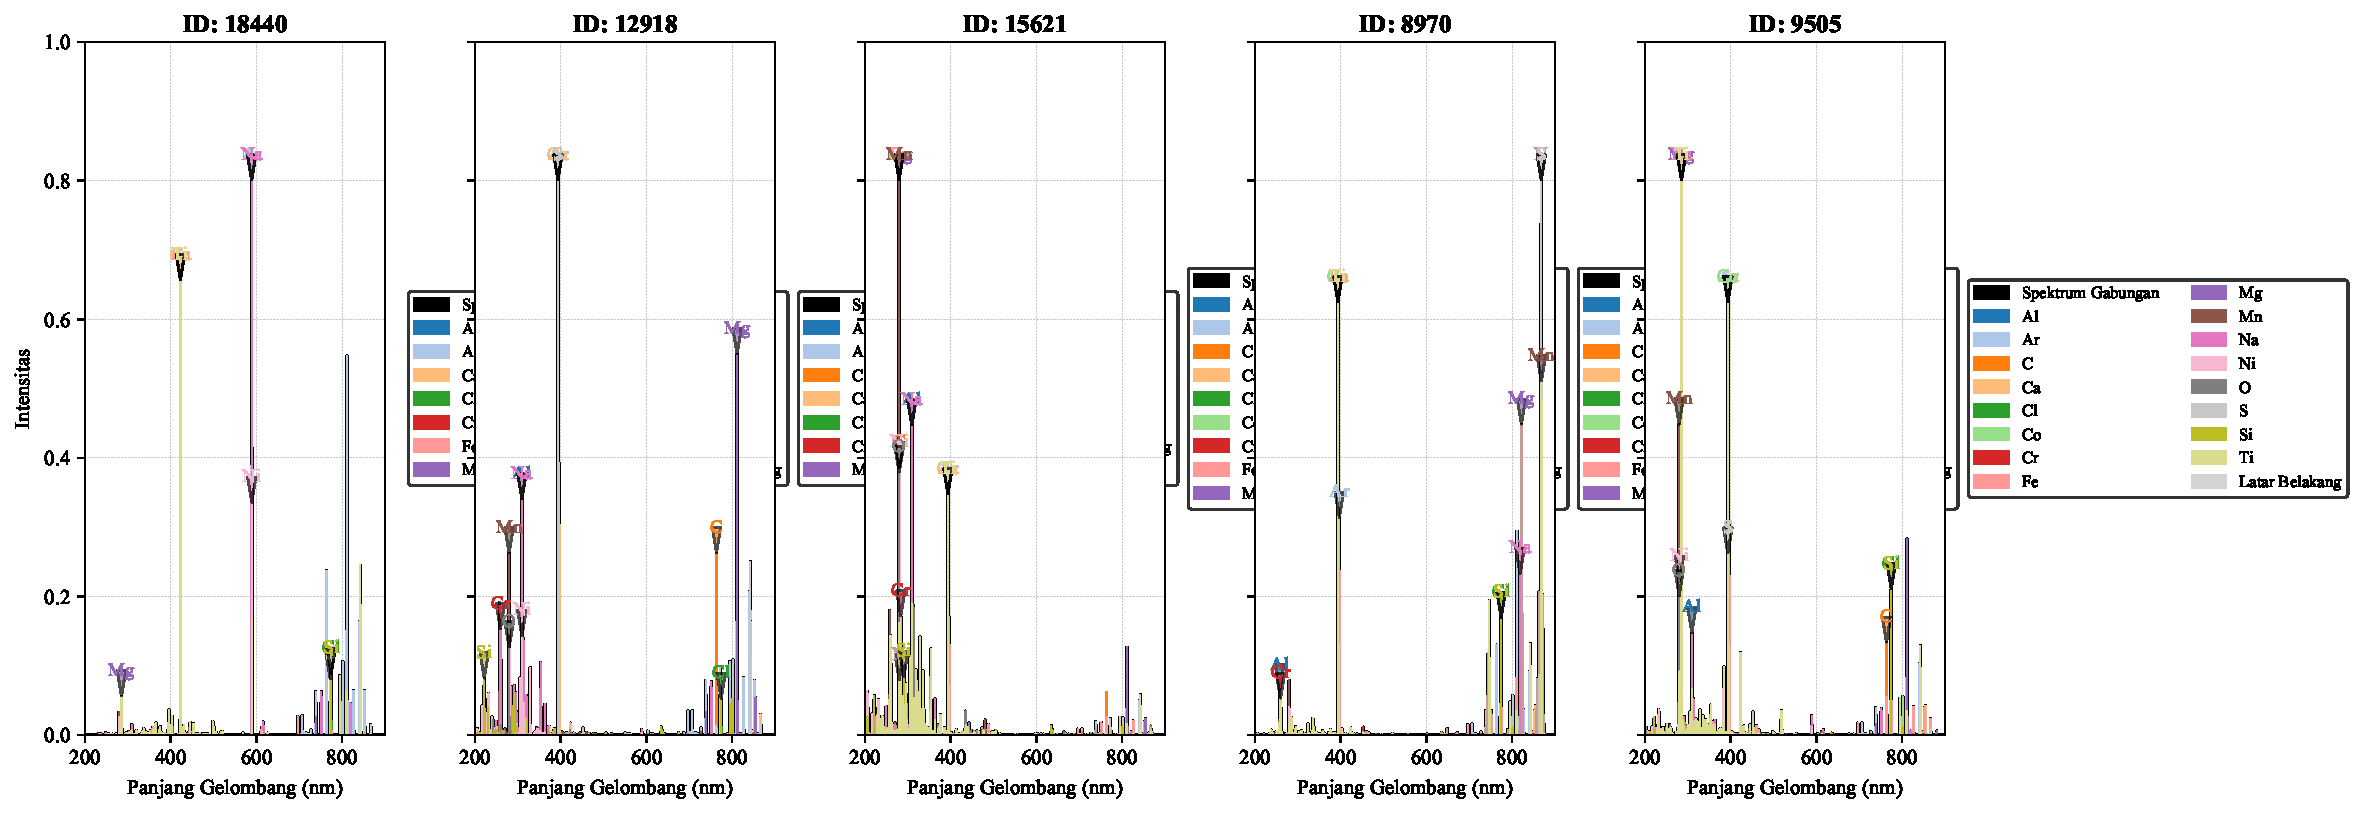
\includegraphics[width=\textwidth]{spectral_plots.pdf}
    \caption{Spectral simulation plots for all samples in a single landscape page.}
    \label{fig:spectrum_all}
\end{figure}

\clearpage

\section{Sample: 8970}
\subsection{Simulation Parameters}
\begin{table}[h!]
    \centering
    \begin{tabular}{ll}
        \toprule
        \textbf{Parameter} & \textbf{Value} \\
        \midrule
        Temperature ($T$) & 6111 \,\si{K} \\
        Electron Density ($n_e$) & 1.32e+14 \,\si{cm^-3} \\
        Total Pixels & 4096 \\
        Signal-to-Noise Ratio (SNR) & 29.52 \\
        \bottomrule
    \end{tabular}
    \caption{Simulation parameters and additional metrics for sample 8970.}
    \label{tab:params_8970}
\end{table}

\subsection{Composition Analysis}
\begin{table}[h!]
    \centering
    \begin{tabular}{lcc}
        \toprule
        \textbf{Element} & \textbf{Initial Composition (\%)} & \textbf{Actual Positions} \\
        \midrule
        Al & 11.67 & 157.0 \\
        Ar & 1.50 & 393.0 \\
        C & 4.75 & 165.0 \\
        Ca & 5.53 & 150.0 \\
        Cl & 4.79 & 12.0 \\
        Co & 1.01 & 864.0 \\
        Cr & 8.53 & 397.0 \\
        Fe & 10.70 & 2325.0 \\
        Mg & 3.60 & 169.0 \\
        Mn & 11.65 & 683.0 \\
        N & 6.52 & 396.0 \\
        Na & 0.29 & 314.0 \\
        Ni & 1.48 & 478.0 \\
        O & 2.81 & 10.0 \\
        S & 9.38 & 25.0 \\
        Si & 11.88 & 216.0 \\
        Ti & 3.89 & 1181.0 \\
        background & N/A & 797.0 \\

        \midrule
        \textbf{Total Positions} & & 8732.0 \\
        \bottomrule
    \end{tabular}
    \caption{Composition analysis for sample 8970.}
    \label{tab:comp_8970}
\end{table}

\subsection{Spectral Plot}
\begin{figure}[h!]
    \centering
    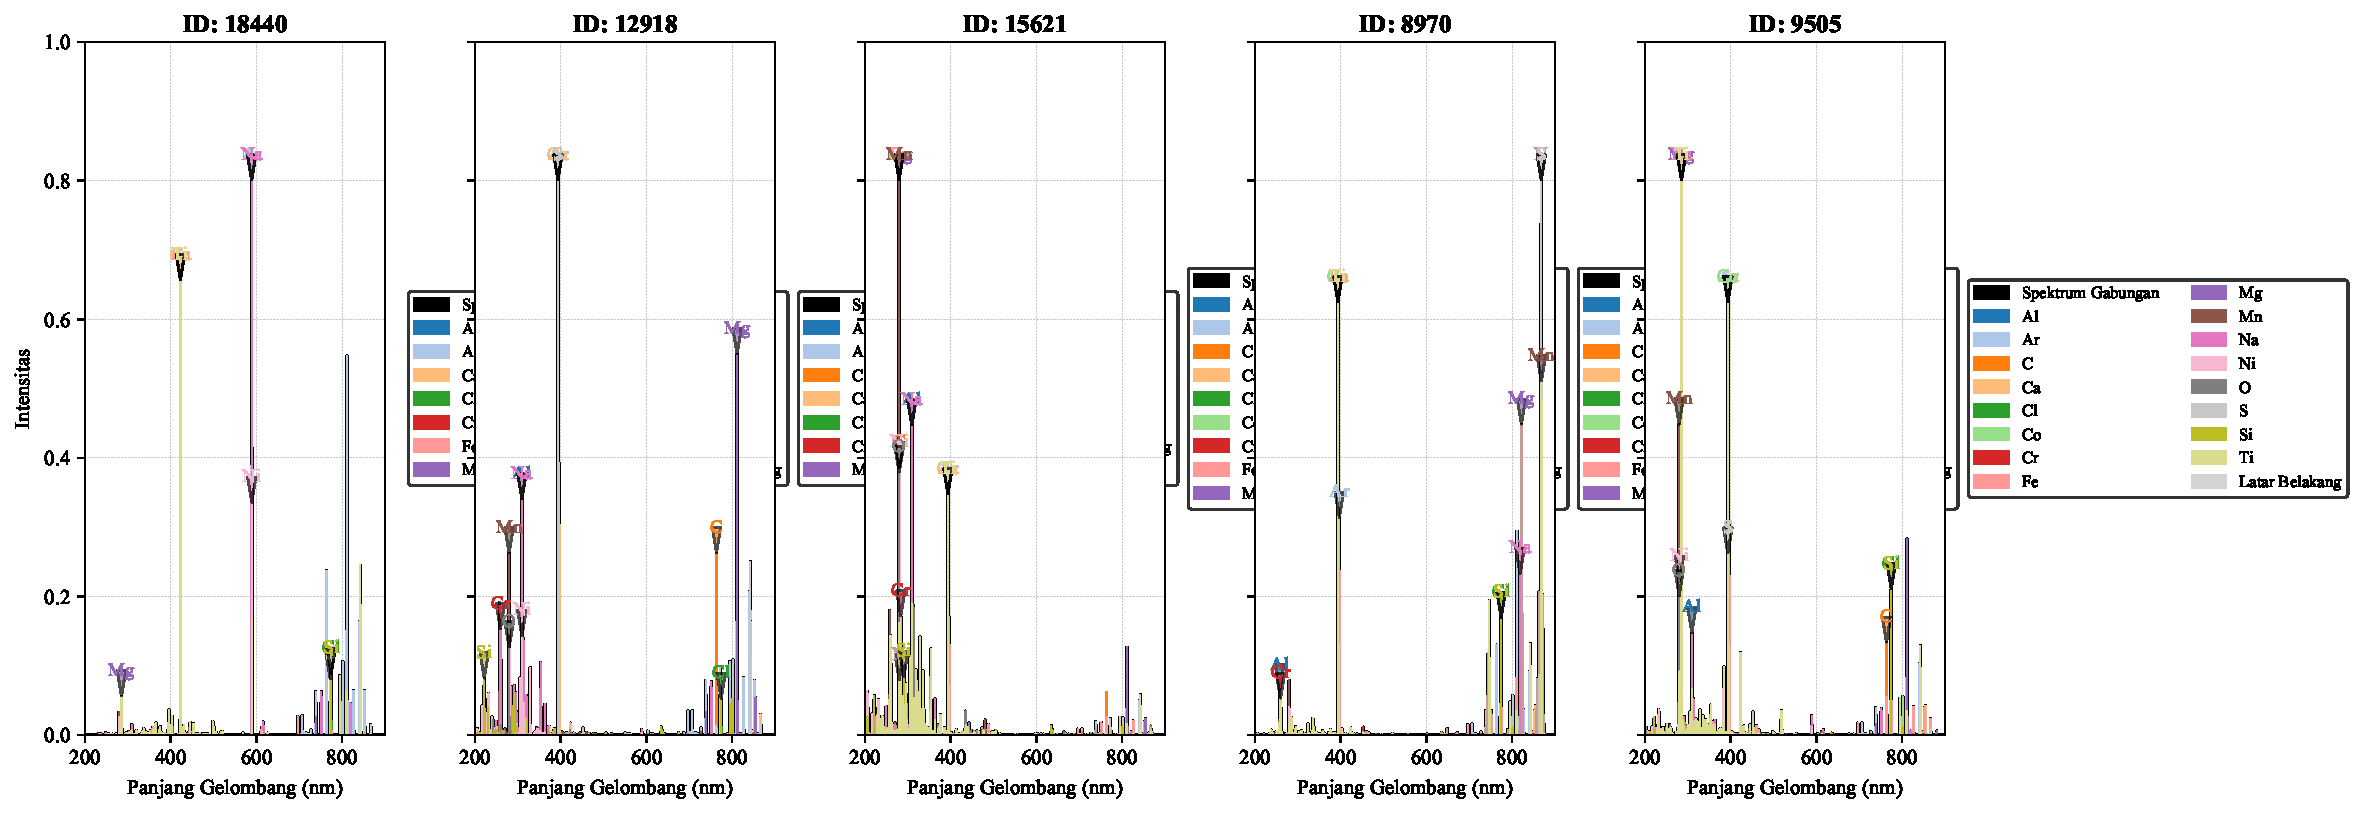
\includegraphics[width=\textwidth]{spectral_plots.pdf}
    \caption{Spectral simulation plots for all samples in a single landscape page.}
    \label{fig:spectrum_all}
\end{figure}

\clearpage

\section{Sample: 9505}
\subsection{Simulation Parameters}
\begin{table}[h!]
    \centering
    \begin{tabular}{ll}
        \toprule
        \textbf{Parameter} & \textbf{Value} \\
        \midrule
        Temperature ($T$) & 9242 \,\si{K} \\
        Electron Density ($n_e$) & 2.26e+17 \,\si{cm^-3} \\
        Total Pixels & 4096 \\
        Signal-to-Noise Ratio (SNR) & 34.35 \\
        \bottomrule
    \end{tabular}
    \caption{Simulation parameters and additional metrics for sample 9505.}
    \label{tab:params_9505}
\end{table}

\subsection{Composition Analysis}
\begin{table}[h!]
    \centering
    \begin{tabular}{lcc}
        \toprule
        \textbf{Element} & \textbf{Initial Composition (\%)} & \textbf{Actual Positions} \\
        \midrule
        Al & 7.86 & 440.0 \\
        Ar & 4.20 & 725.0 \\
        C & 8.20 & 233.0 \\
        Ca & 5.93 & 150.0 \\
        Cl & 13.32 & 18.0 \\
        Co & 3.26 & 1404.0 \\
        Cr & 3.07 & 397.0 \\
        Fe & 2.79 & 2720.0 \\
        Mg & 11.40 & 350.0 \\
        Mn & 1.30 & 706.0 \\
        N & 0.00 & 0.0 \\
        Na & 4.11 & 330.0 \\
        Ni & 10.05 & 478.0 \\
        O & 10.06 & 176.0 \\
        S & 7.10 & 163.0 \\
        Si & 4.33 & 218.0 \\
        Ti & 3.02 & 1183.0 \\
        background & N/A & 474.0 \\

        \midrule
        \textbf{Total Positions} & & 10165.0 \\
        \bottomrule
    \end{tabular}
    \caption{Composition analysis for sample 9505.}
    \label{tab:comp_9505}
\end{table}

\subsection{Spectral Plot}
\begin{figure}[h!]
    \centering
    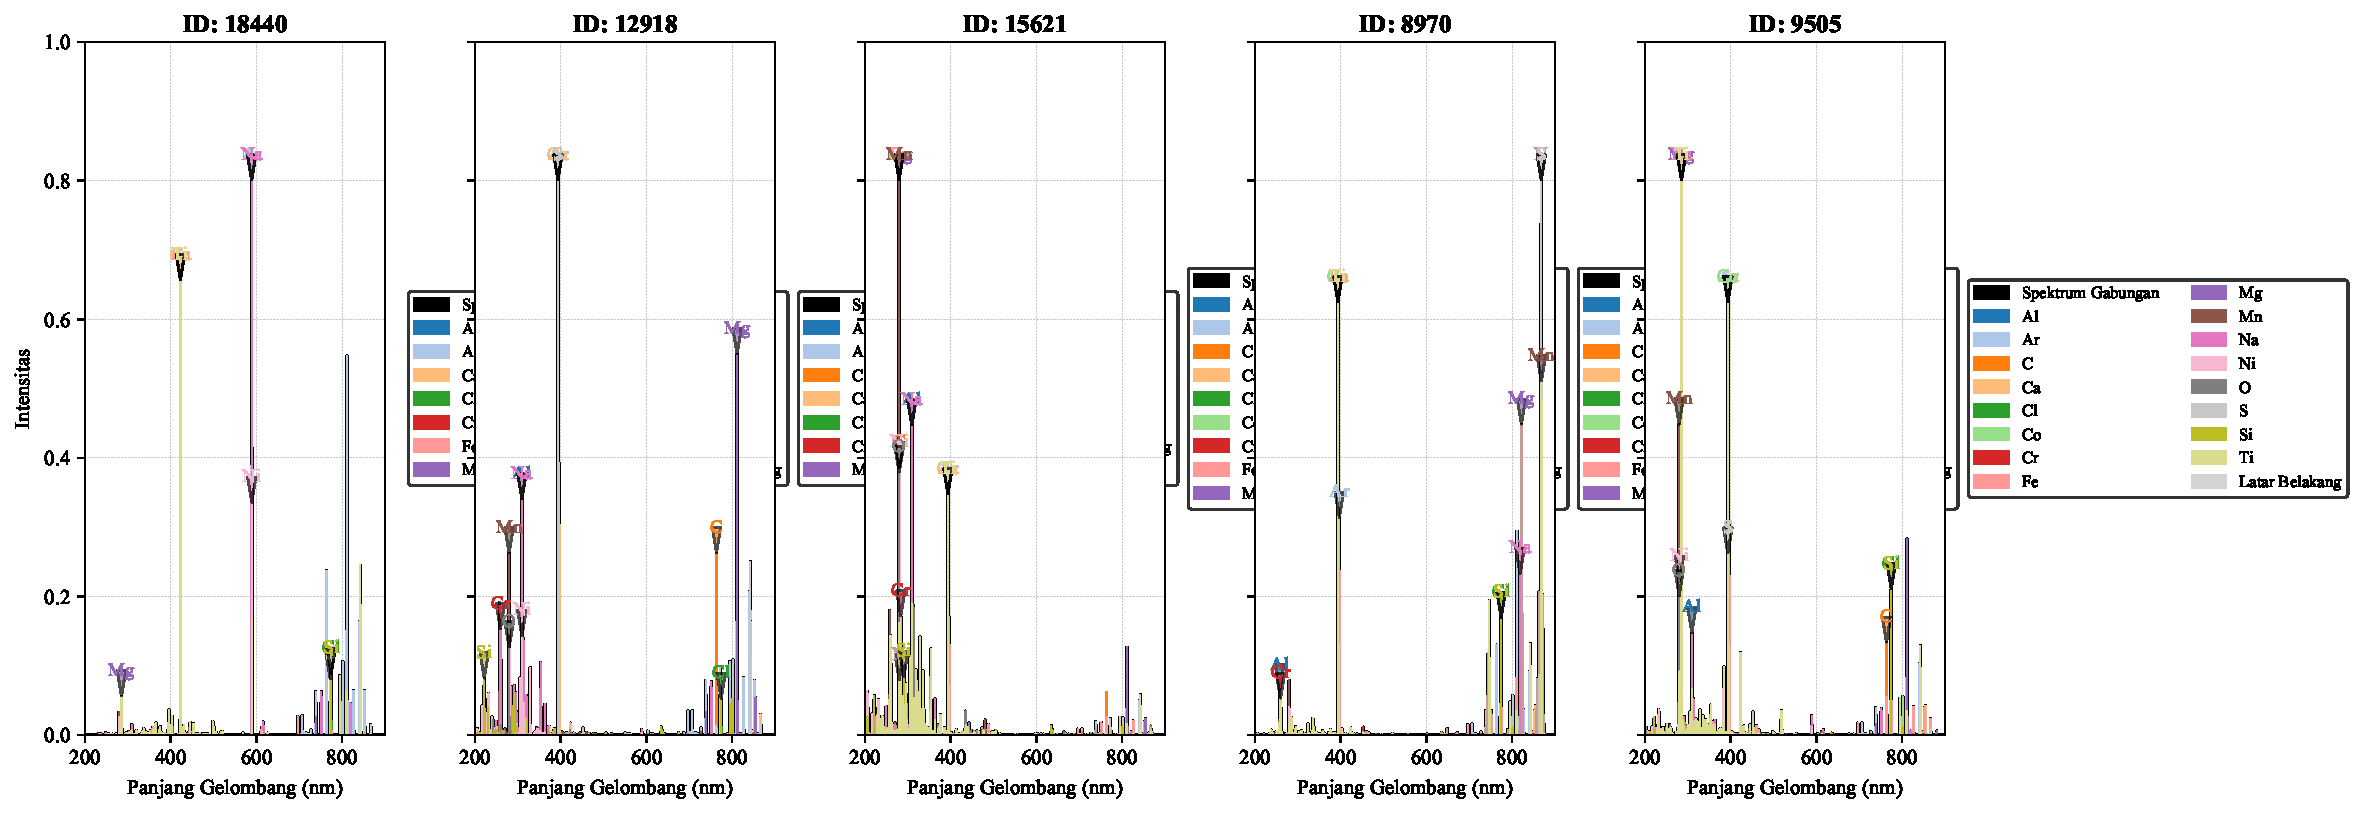
\includegraphics[width=\textwidth]{spectral_plots.pdf}
    \caption{Spectral simulation plots for all samples in a single landscape page.}
    \label{fig:spectrum_all}
\end{figure}

\clearpage

\end{document}
